% ============================================================================
\chapter{Finanças verificáveis: a rodada 0.13}\label{cap:financas}
% ============================================================================

Finanças é o domínio em que ``o número saiu do computador'' vale menos. Um preço que muda quando o cálculo muda de servidor, um \textit{backtest} que olhou o dia seguinte sem querer, a melhor de cinquenta estratégias apresentada como se fosse a única, um livro de ofertas que ninguém de fora consegue auditar: são as dores reais da indústria, e todas são dores de \textbf{verificabilidade}, não de velocidade. Este capítulo descreve como a rodada 0.13 aplica a tese do \autoref{cap:introducao} a esse domínio.

\begin{graduacao}
\textbf{Glossário mínimo.} Uma \emph{mesa} é a equipe (e o sistema) que precifica e negocia instrumentos. \emph{P\&L} é o resultado (\textit{profit and loss}). Um \emph{backtest} simula uma estratégia sobre dados históricos. \emph{Bid} e \emph{ask} são os melhores preços de compra e de venda oferecidos; a diferença é o \emph{spread}. Uma \emph{ordem limitada} só executa ao preço dado ou melhor; uma \emph{ordem a mercado}, ao que houver. HFT (\textit{high-frequency trading}) é a negociação automatizada em escalas de micro a nanossegundos.
\end{graduacao}

% ----------------------------------------------------------------------------
\section{A mesa como arquitetura}\label{sec:fin-mesa}

A \autoref{fig:fin-mesa} mostra o desenho comum a todas as tarefas. O usuário escreve o problema como uma mesa o escreveria --- \code{di1 F26 = 15.02\%}, \code{call S=100 K=100 T=1 r=5\% vol=20\%}, \code{sell 50 @ 101.30 owner=bia} ---; um analisador próprio o lê; um motor o resolve; e a resposta sai com um certificado calculado por um caminho diferente do que a produziu. A mesma entrada chega por quatro portas: a API Elixir (\code{Vapor.Finance.run/2}), a linha de comando (\code{mix vapor.finance}), o console web (\emph{Mercados}) e o servidor MCP, pelo qual um modelo de linguagem pode pedir um cálculo ou submeter uma proposta para conferência.

\begin{figure}[htbp]
\centering
\begin{tikzpicture}[node distance=5mm and 7mm, font=\footnotesize]
\node[box] (api) {API\\Elixir};
\node[box, below=of api] (cli) {\code{mix}\\\code{vapor.finance}};
\node[box, below=of cli] (web) {console\\(Mercados)};
\node[box, below=of web] (mcp) {MCP\\(modelos)};
\node[box, right=10mm of cli, yshift=-5mm] (parse) {texto da mesa\\$\to$ analisador};
\node[box, right=of parse, yshift=10mm] (eng) {motor\\(curva, opção, MC,\\livro, LP\ldots)};
\node[acc, right=of parse, yshift=-10mm] (cert) {certificado\\(outro caminho)};
\node[dark, right=of eng, yshift=-10mm] (ans) {resposta +\\certificado +\\controle};
\node[box, below=8mm of ans] (arc) {arquivo assinado\\(\code{vapor-archive-v1})};
\foreach \n in {api,cli,web,mcp} \draw[arr] (\n.east) -- (parse.west);
\draw[arr] (parse) -- (eng); \draw[arr] (parse) -- (cert); \draw[arr] (eng) -- (ans); \draw[carr] (cert) -- (ans); \draw[arr] (ans) -- (arc);
\draw[arr, dashed] (eng) -- node[lbl, right] {resultado} (cert);
\end{tikzpicture}
\caption{A mesa de finanças: quatro portas, um analisador, um motor e um certificado calculado por outro caminho.}
\label{fig:fin-mesa}
\end{figure}

A \autoref{tab:fin-tarefas} resume as tarefas e o objeto que permite julgar cada resposta. As seções seguintes descrevem cada uma.

\begin{table}[htbp]
\centering
\caption{Tarefas da mesa e o certificado de cada uma}\label{tab:fin-tarefas}
\small
\begin{tabularx}{\textwidth}{@{}lX@{}}
\toprule
\textbf{tarefa} & \textbf{certificado}\\
\midrule
calendário e dinheiro & feriados por regra, iguais ao QuantLib por 89 anos; rateio que soma exatamente\\
curva & todo instrumento reprecificado; \textit{forwards} negativos apontados\\
opções & paridade; gregas contra diferenças finitas; limites de não arbitragem \emph{antes} de resolver; $g(k)$ de Durrleman\\
Monte Carlo & bits = oráculo exato = outra contagem de \textit{threads}; intervalo de 99\% contra a forma fechada\\
risco & Kupiec, Christoffersen, zona de Basileia; tamanho e poder medidos\\
carteira & condições KKT; contribuições de risco iguais aos orçamentos\\
\textit{backtest} & quatro portões: invariância de prefixo, Sharpe deflacionado, PBO, \textit{Reality Check}\\
arbitragem & \emph{ou} o portfólio de arbitragem \emph{ou} os preços de estado, em racionais exatos\\
livro de ofertas & diário SHA-256 + raiz de Merkle; motor ingênuo independente; feed ITCH; FIX\\
sessão de bolsa & os três certificados do livro + a mesma cabeça de \textit{hash} ao repetir\\
microestrutura & teste de reescala do tempo; o artigo reproduzido; forma fechada = ótimo numérico\\
\bottomrule
\end{tabularx}
\end{table}

% ----------------------------------------------------------------------------
\section{Dinheiro exato e calendários por regra}\label{sec:fin-dinheiro}

\paragraph{Dinheiro.} Um valor monetário é um inteiro e uma escala decimal: $\{c = 12345, e = 2\}$ representa 123,45. Soma, subtração e produto são exatos; todo arredondamento é um ato explícito com modo nomeado (\textit{half-even}, \textit{half-up}, \textit{down}, \textit{floor}\ldots), implementado por uma única primitiva testada nos empates dos dois lados do zero. O rateio usa o método do \emph{maior resto} (Hamilton): R\$~100,00 em três partes dá 33,34 + 33,33 + 33,33, e a soma é o total \emph{por construção}; o certificado diz também que cada parte está a menos de uma unidade da sua fração exata. O controle: o mesmo rateio por piso em binary64 perde um centavo (99,99).

O fator da convenção brasileira, $(1 + r)^{\mathrm{DU}/252}$, é calculado com uma raiz inteira em aritmética de inteiros grandes e \emph{truncado} na oitava casa, como faz a ANBIMA. Para $r = 13{,}65\%$ e um dia útil, $(1{,}1365)^{1/252} = 1{,}00050788\ldots$; o módulo \code{decimal} do Python com 60 dígitos concorda --- a decisão na oitava casa não é um acidente de ponto flutuante.

\paragraph{Calendários.} Cada feriado é uma \emph{regra}: data fixa, $n$-ésimo dia da semana, ou festa móvel pelo cômputo gregoriano. A Páscoa sai do algoritmo anônimo de 1876 (Meeus/Jones/Butcher); o Carnaval é a Páscoa menos 48 e 47 dias; a Sexta-feira Santa, menos 2; Corpus Christi, mais 60. Os fechamentos que nenhuma regra produz (11 de setembro de 2001, o furacão Sandy, dias de luto presidencial) são \emph{dados}, cada um com o motivo. A \autoref{tab:calendarios} mostra a conferência contra o QuantLib \cite{quantlib}.

\begin{table}[htbp]
\centering
\caption{Calendários conferidos dia a dia contra o QuantLib 1.43}\label{tab:calendarios}
\small
\begin{tabularx}{\textwidth}{@{}lXr@{}}
\toprule
\textbf{calendário} & \textbf{regras} & \textbf{feriados em dia útil idênticos}\\
\midrule
ANBIMA (= B3) & nacionais + móveis; 20 de novembro desde 2024 (Lei 14.759/2023) & 903 (1990--2078)\\
NYSE & datas observadas; MLK desde 1998; Juneteenth desde 2022; fechamentos especiais & 848\\
TARGET & Sexta Santa, Segunda de Páscoa, 1º de maio e 26 de dezembro desde 2000 & 401\\
\bottomrule
\end{tabularx}
\end{table}

Na primeira comparação, a NYSE divergiu num único dia --- 27/04/1994, o luto pelo presidente Nixon --- e o TARGET em datas anteriores a 2000, quando o sistema não existia. As duas diferenças viraram dado e regra, e o teste passou a exigir igualdade dia a dia. As seis bases de contagem (DU/252, ACT/360, ACT/365F, 30/360, 30E/360, ACT/ACT ISDA) concordam com o QuantLib a $10^{-14}$ nos casos de borda.

\begin{graduacao}
\textbf{Por que dinheiro não é \texttt{double}.} 0,1 não tem representação binária finita. Somar dez vezes 0,10 em binary64 não dá exatamente 1,00, e um rateio feito com pisos em binary64 pode perder um centavo. O erro é minúsculo por operação, mas é um erro \emph{contábil}: o total não fecha. Inteiros com escala decimal fecham por construção.
\end{graduacao}

% ----------------------------------------------------------------------------
\section{Curvas de juros}\label{sec:fin-curvas}

A curva é escrita como uma mesa a escreve (\autoref{fig:fin-curva}). O \textit{bootstrap} põe um nó no último fluxo de cada instrumento e acha, pelo método de Brent, o fator de desconto que o reprecifica, com os nós anteriores fixos. A interpolação é \textit{flat-forward} (log-linear no desconto, a convenção da curva DI) ou linear na taxa zero. Os fluxos seguem as convenções publicadas: o DI1 tem PU $100\,000/(1+r)^{\mathrm{DU}/252}$; a LTN paga 1\,000 no dia útil seguinte ao vencimento; a NTN-F paga cupom semestral $1\,000 \cdot (\sqrt{1{,}1} - 1)$.

\paragraph{O certificado} reprecifica cada instrumento a partir da curva pronta e dá o pior erro relativo ($4{,}5 \cdot 10^{-16}$ na curva DI do exemplo); lista os \textit{forwards} entre nós e \emph{aponta os negativos}. O exemplo ``cotação inconsistente'' (janeiro a 15\%, julho a 9\%) é reprecificado, mas sai com o \textit{forward} negativo nomeado: reprecificar não basta para uma curva ser plausível, e o certificado diz as duas coisas. O controle: o mesmo DI1 contado em dias corridos erra o PU em $2{,}5 \cdot 10^{-3}$. Depósitos simples conferem com o \code{PiecewiseLogLinearDiscount} do QuantLib a $10^{-13}$.

\begin{figure}[htbp]
\centering
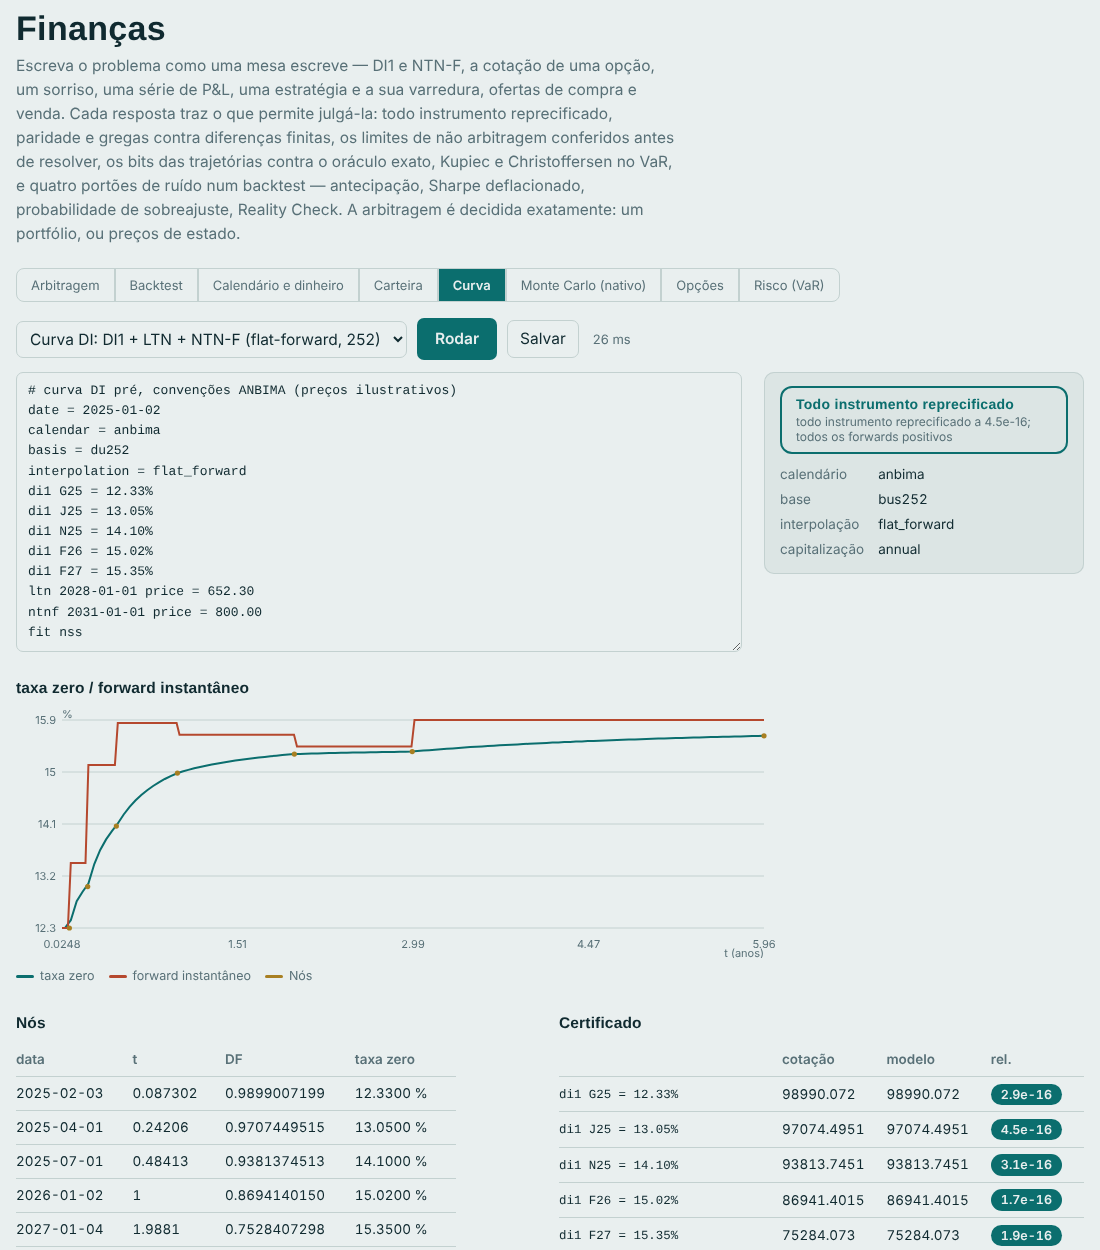
\includegraphics[width=0.82\textwidth]{figuras/console-financas-curva.png}
\caption{Curva DI (DI1 + LTN + NTN-F, \textit{flat-forward}, DU/252) no console: taxa zero, \textit{forward} instantâneo, nós e o certificado de reprecificação.}
\label{fig:fin-curva}
\end{figure}

% ----------------------------------------------------------------------------
\section{Opções}\label{sec:fin-opcoes}

O módulo de opções cobre Black--Scholes--Merton com dividendos \cite{black1973,merton1973}, Black-76, Bachelier (taxas negativas), árvores de Cox--Ross--Rubinstein e Leisen--Reimer \cite{leisen1996}, Heston \cite{heston1993} pela integral de Lewis com a função característica ``\textit{little trap}'' \cite{albrecher2007}, e o sorriso SVI \cite{gatheral2014}. Duas decisões de projeto merecem destaque.

\paragraph{Limites antes de resolver.} A volatilidade implícita é a raiz de $\mathrm{BSM}(\sigma) = p$. Para uma \textit{call}, $\mathrm{BSM}$ é estritamente crescente em $\sigma$ e
\begin{equation}
  \max\!\left(S e^{-qT} - K e^{-rT}, 0\right) < \mathrm{BSM}(\sigma) < S e^{-qT}, \qquad \sigma \in (0, \infty).
  \label{eq:limites}
\end{equation}
Um preço fora desse intervalo não tem volatilidade implícita --- e não é ``mal condicionado'': é uma arbitragem. O \vapor{} confere os limites \emph{antes} de chamar o \textit{solver} e recusa com o limite violado; dentro deles, devolve o erro de reprecificação, a vega e quanto um \textit{tick} de preço move $\sigma$ (o condicionamento, em unidades de mercado).

\paragraph{Arbitragem de borboleta no sorriso.} Uma fatia do SVI dá a variância total $w(k)$ em função do \textit{log-strike} $k$. \citeonline{gatheral2014} mostram que a densidade neutra ao risco implícita é não negativa se e só se
\begin{equation}
  g(k) = \left(1 - \frac{k\, w'(k)}{2\, w(k)}\right)^{\!2} - \frac{w'(k)^2}{4}\left(\frac{1}{w(k)} + \frac{1}{4}\right) + \frac{w''(k)}{2} \;\geq\; 0.
  \label{eq:durrleman}
\end{equation}
O \vapor{} avalia $g$ numa grade fina e devolve o intervalo em que ela é negativa. A fatia que \citeonline{gatheral2014} atribuem a Vogt --- o exemplo clássico de arbitragem de borboleta --- é detectada ($g$ mínimo $-0{,}033$ em $k \in [0{,}645;\, 1{,}255]$); um sorriso calmo ajustado sai com $g \geq 0$ (\autoref{fig:fin-sorriso}).

\begin{figure}[htbp]
\centering
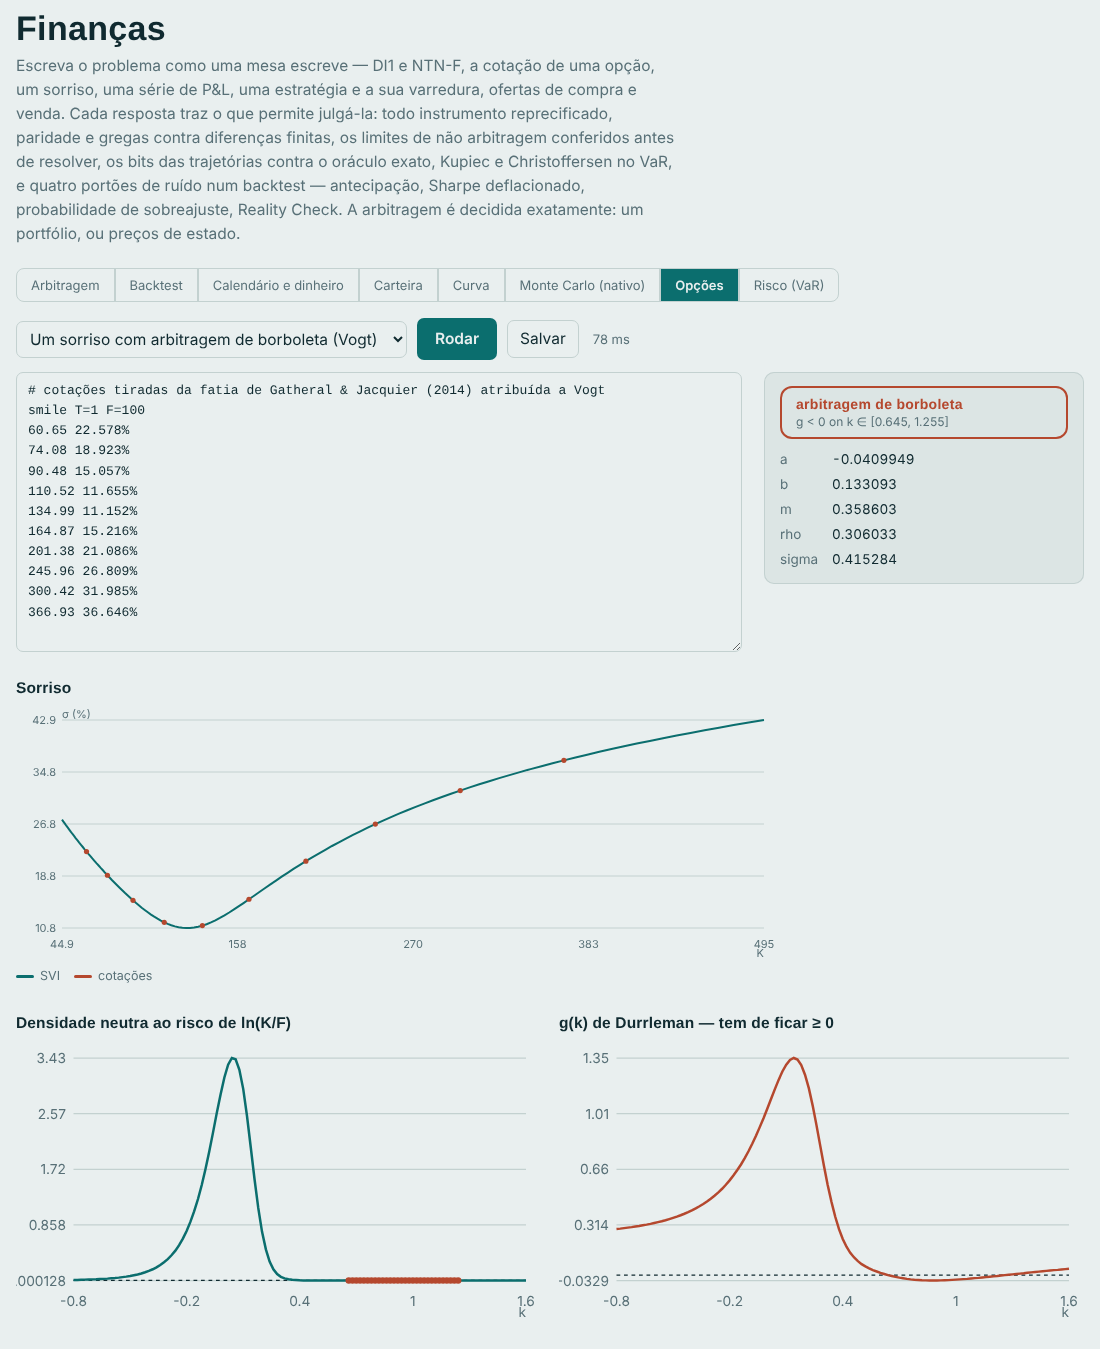
\includegraphics[width=0.82\textwidth]{figuras/console-financas-sorriso.png}
\caption{O sorriso de Vogt: o ajuste SVI, a densidade neutra ao risco (negativa onde há arbitragem) e $g(k)$ de Durrleman abaixo de zero.}
\label{fig:fin-sorriso}
\end{figure}

\paragraph{Contra o QuantLib.} BSM, $\Delta$ e $\Gamma$ a $10^{-12}$, vega a $10^{-10}$; americana de Leisen--Reimer com 801 passos a $10^{-10}$ (4,486076, a \textit{put} da tabela~1 de \citeonline{longstaff2001}); Heston a $10^{-9}$ (o integrador adaptativo de Gauss--Kronrod do QuantLib e a Gauss--Legendre composta daqui concordam até a nona casa). O CRR daqui é o de livro-texto e o do QuantLib usa a aproximação aditiva em log; diferem em $1{,}6 \cdot 10^{-5}$, e a documentação diz qual é qual. O LSM de \citeonline{longstaff2001} sobre a mesma \textit{put} dá $4{,}4788 \pm 0{,}0143$ (o artigo: 4,472).

% ----------------------------------------------------------------------------
\section{Monte Carlo compilado para o núcleo}\label{sec:fin-mc}

A dor: um número de risco que muda quando o cálculo muda de máquina, de contagem de \textit{threads} ou para uma GPU --- reduções paralelas em outra ordem, uma FMA aqui e não ali, outro $\exp$. A resposta do \vapor{}: escrever o passo da trajetória como termos da álgebra e herdar a garantia central.

\paragraph{O passo.} Para o log-preço $L$, com $\mu\Delta = (r - q - \sigma^2/2)\Delta$ e $\sigma\sqrt{\Delta}$ pré-calculados, o programa recorrente atualiza, por trajetória e por passo,
\begin{equation}
  L \leftarrow L + \mu\Delta + \sigma\sqrt{\Delta}\,\Phi^{-1}(u), \quad A \leftarrow A + e^{L}, \quad G \leftarrow G + L, \quad v \leftarrow v \cdot [L > \ln(B/S_0)],
  \label{eq:passo-mc}
\end{equation}
em que $A$ e $G$ acumulam as médias aritmética e geométrica (opções asiáticas) e $v$ marca as trajetórias vivas acima de uma barreira $B$. $\Phi^{-1}$ é o algoritmo AS241 de \citeonline{wichura1988} (PPND7, 7 dígitos --- o que binary32 comporta), com $\log$ e $\mathrm{rsqrt}$ canônicos.

\paragraph{O gerador dentro da álgebra.} Para que a trajetória inteira rode no worker, o gerador também precisa ser termo da álgebra --- e exato em binary32. O \vapor{} usa o gerador de \citeonline{wichmann1982}: três geradores de Lehmer
\begin{equation}
  s_1 \leftarrow 171\, s_1 \bmod 30269, \quad s_2 \leftarrow 172\, s_2 \bmod 30307, \quad s_3 \leftarrow 170\, s_3 \bmod 30323,
\end{equation}
combinados como $u = (s_1/30269 + s_2/30307 + s_3/30323) \bmod 1$.

\begin{proposicao}\label{prop:wh}
Cada atualização de estado do gerador de Wichmann--Hill é calculada exatamente em binary32 pelo programa
\[
p = a \cdot s,\qquad q = \lfloor p \oslash m \rfloor,\qquad s' = p - m \cdot q,
\]
em que $\oslash$ é a divisão corretamente arredondada e $\lfloor y \rfloor$ é calculado por $r = (y \oplus 2^{23}) \ominus 2^{23}$, seguido de $r \ominus 1$ quando $r > y$.
\end{proposicao}

\begin{proof}[Esboço]
Os produtos $a \cdot s$ são inteiros menores que $171 \cdot 30268 = 5\,175\,828 < 2^{23}$ (e analogamente para os outros dois), logo representáveis exatamente com 24 bits de significando: $p$ é exato. Para $0 \leq y < 2^{23}$, somar $2^{23}$ leva $y$ ao binade $[2^{23}, 2^{24})$, em que o ulp é 1; o arredondamento ao mais próximo produz o inteiro mais próximo de $y$, e subtrair $2^{23}$ é exato (Sterbenz). Se o arredondamento subiu, $r > y$ e a correção desce um. O quociente $p/m$ nunca é inteiro (pois $m$ é primo e $0 < s < m$) e, para estes três módulos, nunca arredonda para o inteiro seguinte --- o que se confere exaustivamente, para os cerca de 91 mil estados possíveis ---, de modo que $\lfloor p \oslash m \rfloor = \lfloor p/m \rfloor$; dois seletores no programa corrigem $s'$ para $[0, m)$ por segurança. Finalmente, $m \cdot q \leq p < 2^{23}$ é exato e a subtração de inteiros abaixo de $2^{23}$ também.
\end{proof}

O resultado é que a BEAM só semeia: sementes, geração, transformação normal, passo e acumulação rodam no worker, com os mesmos bits em todo substrato.

\paragraph{Certificados, na mesma resposta.} (i) A primeira chamada, compilada para 64 pistas e rodada pelo \emph{oráculo exato}, é igual bit a bit às 64 primeiras pistas do worker. (ii) A simulação inteira, repetida num worker com 2 \textit{threads}, dá os mesmos bits. (iii) As mesmas uniformes em binary64 na BEAM, com $\Phi^{-1}$ de precisão total, diferem no máximo $2 \cdot 10^{-5}$ no \textit{payoff}. (iv) O intervalo de 99\% contém a forma fechada --- BSM para a europeia, \citeonline{kemna1990} para a asiática geométrica discreta. (v) A asiática aritmética usa a geométrica como variável de controle, com variância dividida por cerca de 1\,300. \textbf{O controle:} esquecer o $-\sigma^2/2$ de Itô em $\mu\Delta$ dá $z = 8{,}7$ --- o estimador viciado é pego, não promediado.

\begin{figure}[htbp]
\centering
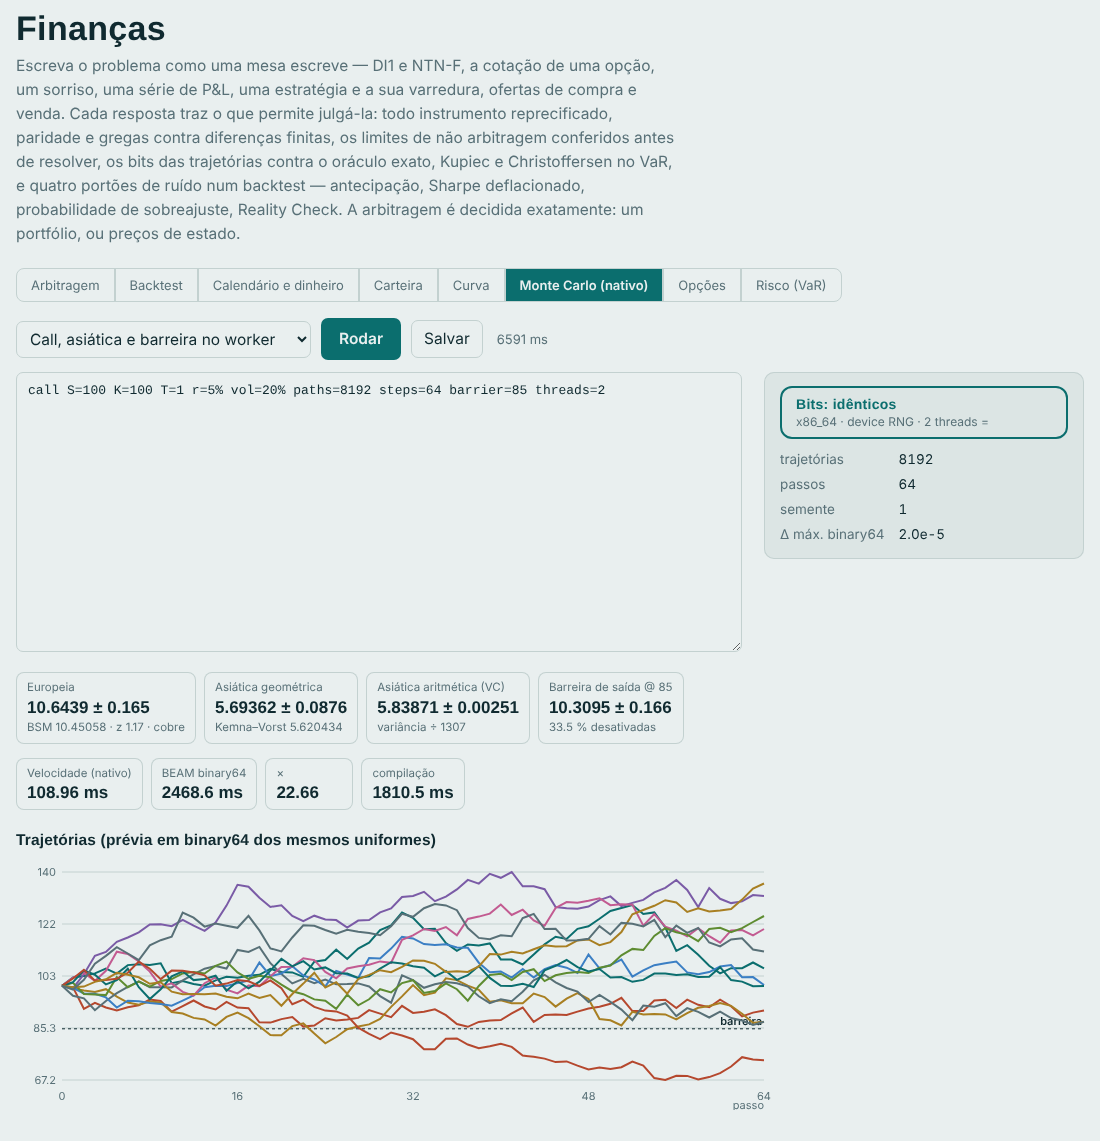
\includegraphics[width=0.82\textwidth]{figuras/console-financas-montecarlo.png}
\caption{Monte Carlo no worker nativo: europeia, asiáticas e barreira, com o selo de bits idênticos (oráculo e 2 \textit{threads}) e a comparação com a BEAM em binary64.}
\label{fig:fin-mc}
\end{figure}

\paragraph{Desempenho.} Numa máquina de 2 vCPUs com AVX-512, um núcleo do worker: 8\,192 trajetórias $\times$ 64 passos em 125~ms, contra 750~ms estimados para a BEAM em binary64 (6$\times$); 16\,384 $\times$ 32 em 86~ms contra 1\,950~ms (23$\times$). A compilação custa cerca de 0,6~s por passo desenrolado e por ISA, por causa do verificador de alocação quadrático (\autoref{sec:inov-alocacao}); por isso o programa tem um passo por chamada e compila só para a ISA da máquina.

\paragraph{Limite.} Wichmann--Hill é um gerador antigo: período de cerca de $7 \cdot 10^{12}$ e falha em baterias modernas como a BigCrush \cite{lecuyer2007}. Serve à precificação, não à criptografia nem a estudos de cauda extrema; a opção \code{rng: :host} usa \textit{splitmix64} na BEAM e compara.

\begin{doutorado}
\textbf{Geradores modernos exatos em binary32.} A restrição ``produtos abaixo de $2^{23}$'' exclui os geradores de qualidade atual (PCG, Philox, xoshiro), que dependem de aritmética inteira de 32 ou 64 bits. A álgebra do \vapor{} tem um gerador \code{gemm\_i8} em $\mathbb{Z}/2^{32}\mathbb{Z}$, com paridade inteira provada em Lean. Fica em aberto se um gerador contrabaseado como o Philox \cite{salmon2011} pode ser expresso com esses operadores inteiros, mantendo a exatidão e a igualdade em GPU, e qual o custo comparado ao Wichmann--Hill em ponto flutuante.
\end{doutorado}

% ----------------------------------------------------------------------------
\section{Risco de mercado e carteiras}\label{sec:fin-risco}

O VaR é calculado pelos métodos histórico, normal, Cornish--Fisher e EWMA ($\lambda = 0{,}94$), em janela móvel, e testado. Se $x$ exceções ocorrem em $n$ dias para um VaR de cobertura $1 - p$, a estatística de \citeonline{kupiec1995} é
\begin{equation}
  \mathrm{LR}_{\mathrm{pof}} = -2 \ln\!\left[(1-p)^{n-x} p^{x}\right] + 2 \ln\!\left[\left(1 - \tfrac{x}{n}\right)^{n-x}\left(\tfrac{x}{n}\right)^{x}\right] \;\sim\; \chi^2_1,
\end{equation}
e a de \citeonline{christoffersen1998} testa, por uma cadeia de Markov de dois estados, se as exceções se agrupam. A zona de Basileia (verde 0--4, amarela 5--9, vermelha $\geq$ 10 exceções em 250 dias a 99\%) acompanha \cite{basel1996}.

\paragraph{Tamanho e poder.} Um teste que nunca rejeita é tão suspeito quanto um que sempre rejeita. O \vapor{} mede o \emph{tamanho} do Kupiec sorteando exceções a exatamente 1\% em 400 séries (rejeita em 1,5--10\% delas) e o seu \emph{poder} numa série de retornos $t$ de Student com $\nu = 3$: o VaR normal é rejeitado ($p = 0{,}038$) e o histórico não ($p = 0{,}43$) (\autoref{fig:fin-var}).

\begin{figure}[htbp]
\centering
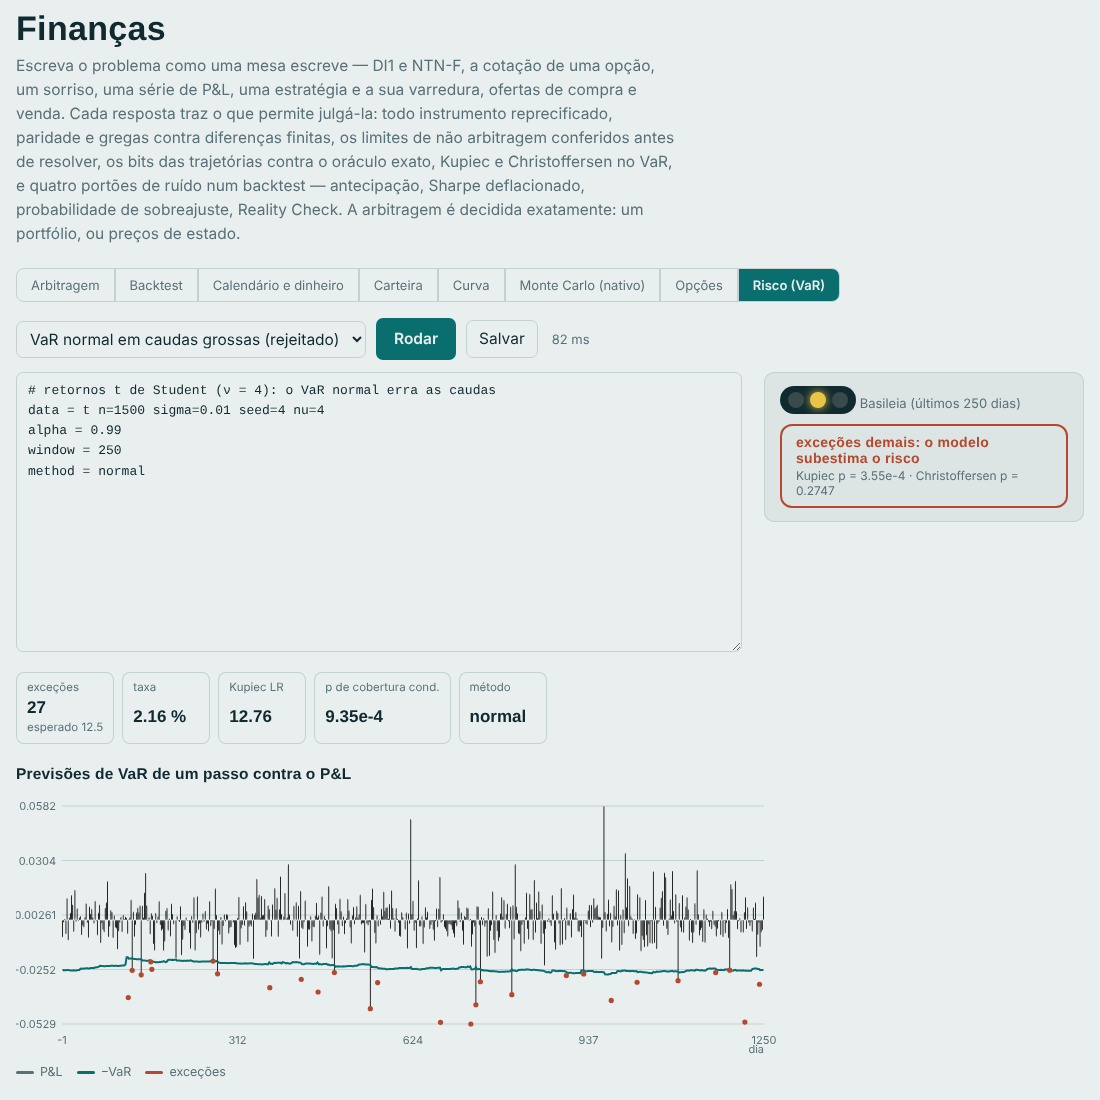
\includegraphics[width=0.82\textwidth]{figuras/console-financas-var.png}
\caption{VaR normal em caudas grossas: as previsões de um passo, as exceções, os testes de Kupiec e Christoffersen e a zona de Basileia.}
\label{fig:fin-var}
\end{figure}

\paragraph{Carteiras.} Covariância encolhida de \citeonline{ledoit2004}; \emph{variância mínima só compra} por conjunto ativo, com as condições KKT como certificado (estacionaridade abaixo de $10^{-12}$, multiplicadores com o sinal certo); \emph{paridade de risco} por Newton na formulação convexa de \citeonline{spinu2013}, com contribuições iguais aos orçamentos a $10^{-12}$; e HRP de \citeonline{lopezdeprado2016}.

% ----------------------------------------------------------------------------
\section{\textit{Backtests} com portões de ruído}\label{sec:fin-backtest}

Um \textit{backtest} é uma máquina de produzir índices de Sharpe; tentando variantes bastantes, uma parecerá boa sobre puro ruído. As duas falhas silenciosas da indústria são a \textbf{antecipação} (o sinal usou informação que não teria) e a \textbf{seleção} (a melhor de muitas tentativas apresentada como a única) \cite{bailey2014pbo,harvey2016}. O \vapor{} trata as duas com quatro portões.

A estratégia é escrita numa linguagem pequena:
\begin{lstlisting}
data = ar1 n=5040 phi=0.15 sigma=0.01 seed=3
sweep k = 1..3
signal = sign(sma(ret(close), k))
cost = 1bp
\end{lstlisting}
Os operadores são causais (\code{lag}, \code{diff}, \code{ret}, \code{sma}, \code{ema}, \code{std}, \code{zscore}, \code{rsi}, \code{sign}, \code{if}\ldots), mas a linguagem aceita, porque as pessoas os escrevem, três que espiam: \code{lead}, \code{center} e \code{normalize} pela amostra inteira. A posição em $(t, t+1]$ é o sinal em $t$; o custo incide sobre $|\Delta\text{posição}|$.

\subsection{Portão 1: invariância de prefixo}

\begin{definicao}[Causalidade observável]
Seja $f$ o \textit{pipeline} que leva uma série de preços $x_{0..n}$ a uma série de sinais $f(x)_{0..n}$. Diz-se que $f$ é \emph{causal} se, para todo $c \leq n$ e todo $t \leq c$, $f(x_{0..c})_t = f(x_{0..n})_t$.
\end{definicao}

\begin{proposicao}\label{prop:prefixo}
Se $f$ é causal, então para qualquer conjunto de cortes $C$ o teste ``$f(x_{0..c})_{0..c} = f(x_{0..n})_{0..c}$ bit a bit para todo $c \in C$'' aceita. Reciprocamente, se o teste rejeita em $c$, existe $t \leq c$ em que o sinal calculado com a história inteira difere do que seria calculado com os dados disponíveis em $c$: $f$ usa informação posterior a $c$.
\end{proposicao}

A proposição é imediata, e é o seu caráter de \emph{caixa-preta} que a torna útil: o teste não precisa conhecer nem confiar nos operadores --- trata o \textit{pipeline} inteiro, inclusive o analisador e o avaliador, como função. Um primeiro rascunho da ideia conferia só os operadores, e teria deixado passar o \code{center}, que é causal em cada passo e não causal no todo (a média é da amostra inteira). Por isso o teste é sobre o resultado, não sobre a gramática. A igualdade é bit a bit porque o avaliador é determinístico; com aritmética não reprodutível, seria preciso uma tolerância, e uma antecipação pequena poderia se esconder nela. O \vapor{} usa oito cortes e devolve o \emph{dia} em que o sinal muda.

\begin{mestrado}
\textbf{Completude.} O teste é correto (nunca acusa um \textit{pipeline} causal) mas não completo: uma antecipação que só se manifeste entre dois cortes, ou que mude o sinal sem mudar o seu valor arredondado, passa. Com $C = \{0, \ldots, n\}$ o teste é completo para a definição acima, ao custo de $n$ avaliações. Os oito cortes são um compromisso; como o custo de cada avaliação é linear, cortes adicionais podem ser pedidos.
\end{mestrado}

\subsection{Portões 2--4: seleção}

O \textbf{Sharpe deflacionado} \cite{bailey2014dsr} é a probabilidade de o Sharpe verdadeiro exceder o máximo esperado de $N$ tentativas sem habilidade:
\begin{equation}
  \mathrm{DSR} = \Phi\!\left(\frac{(\widehat{SR} - SR_0)\sqrt{T-1}}{\sqrt{1 - \hat\gamma_3 \widehat{SR} + \frac{\hat\gamma_4 - 1}{4}\widehat{SR}^2}}\right),
\end{equation}
\begin{equation}
  SR_0 = \sqrt{V}\left[(1-\gamma)\,\Phi^{-1}\!\left(1 - \tfrac{1}{N}\right) + \gamma\, \Phi^{-1}\!\left(1 - \tfrac{1}{N e}\right)\right],
\end{equation}
em que $V$ é a variância dos Sharpes entre tentativas, $\gamma \approx 0{,}5772$ é a constante de Euler--Mascheroni e $\hat\gamma_3, \hat\gamma_4$ são assimetria e curtose. $N$ inclui as tentativas declaradas antes do arquivo (\code{trials =}). A \textbf{probabilidade de sobreajuste} (PBO) por validação cruzada combinatória \cite{bailey2014pbo} divide a série em 16 blocos e, nas $\binom{16}{8} = 12\,870$ metades, mede com que frequência o campeão dentro da amostra cai abaixo da mediana fora dela. O \textbf{\textit{Reality Check}} de \citeonline{white2000} testa se a melhor estratégia supera a nula com o \textit{bootstrap} estacionário de \citeonline{politis1994}.

\paragraph{Medido.} O melhor de 30 cruzamentos de médias sobre um passeio aleatório tem Sharpe positivo e DSR 0,10 --- reprovado (\autoref{fig:fin-backtest}). O sinal plantado (momento sobre AR(1) com $\phi = 0{,}15$) passa os quatro portões (DSR 1,0; PBO $< 0{,}5$; \textit{Reality Check} $p < 0{,}05$). \code{sign(lead(close) - close)} tem Sharpe anual 20 e é pego no dia 89.

\begin{figure}[htbp]
\centering
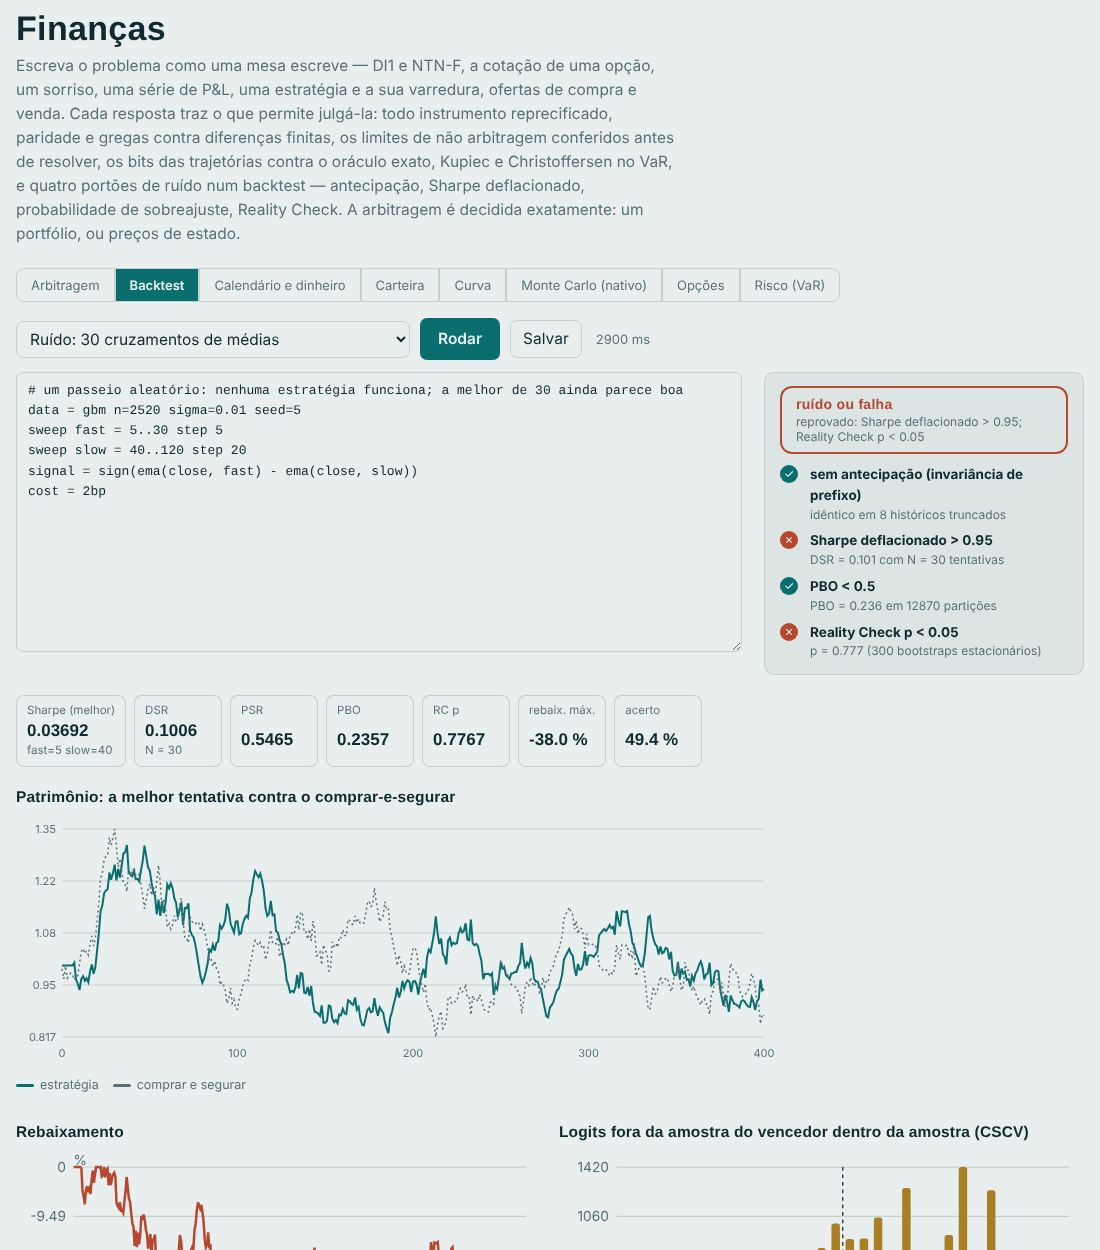
\includegraphics[width=0.82\textwidth]{figuras/console-financas-backtest.png}
\caption{Trinta cruzamentos de médias sobre ruído: o melhor parece bom, e os portões dizem que é ruído (DSR 0,10; \textit{Reality Check} $p = 0{,}78$).}
\label{fig:fin-backtest}
\end{figure}

% ----------------------------------------------------------------------------
\section{Arbitragem decidida exatamente}\label{sec:fin-arbitragem}

\begin{proposicao}[Lema de Farkas, forma de mercado]\label{prop:farkas}
Sejam $n$ ativos com pagamentos $X \in \mathbb{Q}^{n \times S}$ em $S$ estados e cotações $\mathrm{bid}_i \leq \mathrm{ask}_i$. Exatamente uma das alternativas vale:
\begin{enumerate}
  \item existe um portfólio --- compras $b \geq 0$ ao \textit{ask} e vendas $s \geq 0$ ao \textit{bid} --- com custo $\mathrm{ask}^\top b - \mathrm{bid}^\top s \leq 0$, pagamento $X^\top(b - s) \geq 0$ em todo estado, e pelo menos uma das desigualdades estrita;
  \item existem preços de estado $\psi \in \mathbb{Q}^S$, $\psi > 0$, com $\mathrm{bid}_i \leq (X\psi)_i \leq \mathrm{ask}_i$ para todo $i$.
\end{enumerate}
\end{proposicao}

É o teorema fundamental da precificação \cite{harrison1979,jouini1995} visto como teorema da alternativa \cite{farkas1902}. O \vapor{} acha os dois lados com um \textbf{simplex racional exato} (duas fases, regra de Bland contra ciclagem) e devolve o objeto que prova a alternativa encontrada, conferido \emph{só por multiplicação} de racionais:
\begin{itemize}
  \item uma arbitragem: o portfólio, o custo e o pagamento em cada estado. No exemplo da \textit{call} mal precificada, vender um título, comprar 1/90 da ação e vender 1/60 da \textit{call} recebe 1/15 hoje e paga 0 nos dois estados;
  \item ausência de arbitragem: o vetor $\psi > 0$ --- $(1/2,\, 9/20)$ no binomial do exemplo.
\end{itemize}

\begin{mestrado}
\textbf{Por que racionais.} Em ponto flutuante, a decisão entre as duas alternativas é instável na fronteira: um custo de $-10^{-17}$ é arbitragem ou erro de arredondamento? Em racionais, a resposta é exata, e o certificado é conferido por quem quiser com aritmética de inteiros. O custo é que coeficientes irracionais (como $e^{-rT}$) entram arredondados a 15 casas --- e a resposta diz isso. O mesmo simplex racional, com certificados dual, de Farkas e de raio ilimitado, resolve qualquer programa linear na mesa de lógica (\code{maximize}/\code{minimize}), fechando um item da lista de pendências da rodada 0.12.
\end{mestrado}

\paragraph{\textit{Calls} entre \textit{strikes}.} Para cotações de \textit{calls} num vencimento, os estados são 0, cada \textit{strike}, $2K_{\max}$ e a \emph{inclinação} além dele. Como o pagamento de qualquer combinação estática é linear por partes com vértices nos \textit{strikes}, conferir os vértices e a inclinação confere todo preço terminal: a decisão é completa para portfólios estáticos (\autoref{fig:fin-arb}). Câmbio: todos os ciclos simples de até cinco conversões, com o produto das taxas em racionais.

\begin{figure}[htbp]
\centering
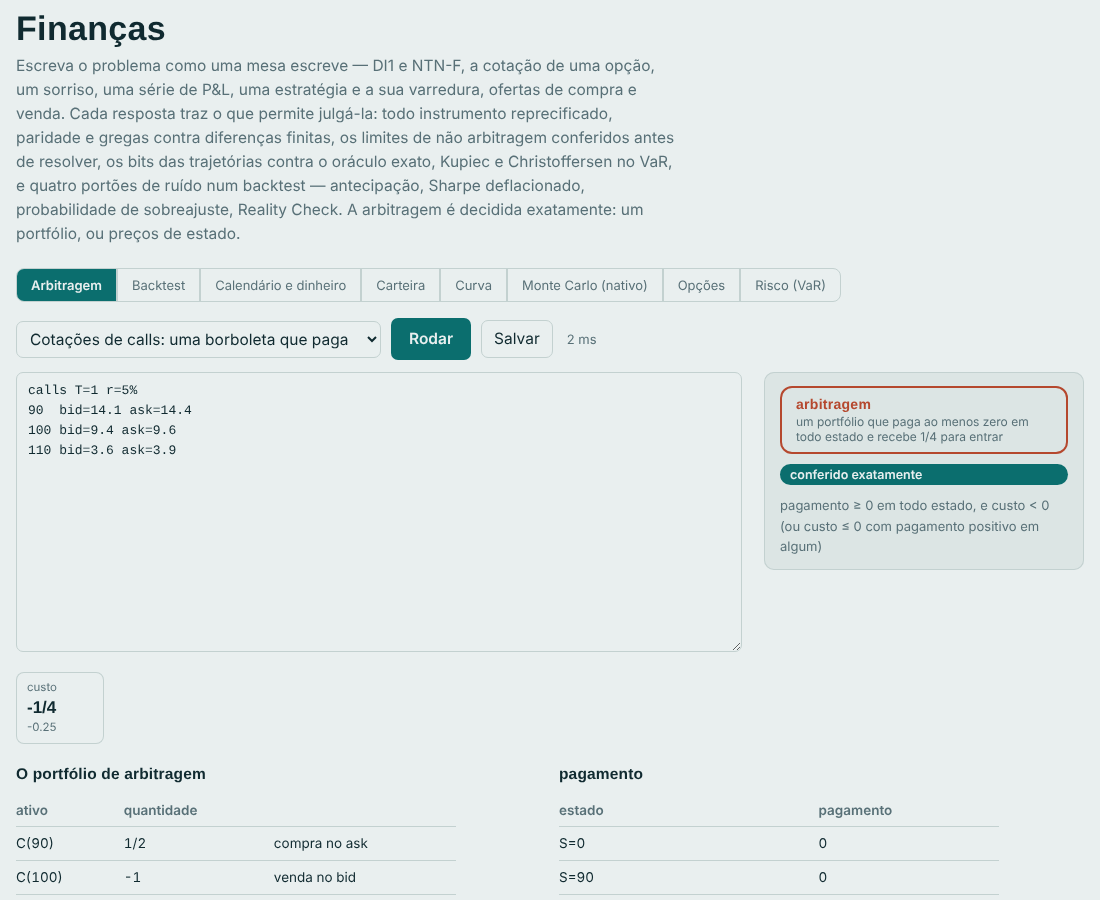
\includegraphics[width=0.82\textwidth]{figuras/console-financas-arbitragem.png}
\caption{Cotações de \textit{calls} com uma borboleta que paga: o portfólio de arbitragem, o custo exato e o pagamento em cada vértice.}
\label{fig:fin-arb}
\end{figure}

\paragraph{Humano ou IA no loop.} A ferramenta MCP \code{arbitrage\_check} recebe a \emph{proposta} de qualquer um --- um portfólio que alguém diz ser arbitragem, ou preços de estado que alguém diz provarem que não há --- e só a aritmética exata decide. O controle do teste: ``compre a ação e venda a \textit{call}'' paga nos dois estados mas custa 86,5 --- não é arbitragem, e a mesa diz por quê.

% ----------------------------------------------------------------------------
\section{O livro de ofertas como objeto verificável}\label{sec:fin-livro}

O motor de casamento implementa prioridade preço--tempo; ordens limitadas e a mercado; validades GTC, IOC e FOK; \textit{post-only}; cancelamento; alteração (reduzir a quantidade no mesmo preço mantém a prioridade; qualquer outra mudança é cancelar e substituir); prevenção de autonegociação; e \textit{kill switch} por dono. Preços são \textit{ticks} inteiros e quantidades são inteiras: nada arredonda. O motor é uma \textbf{função pura} $(\text{livro}, \text{evento}) \mapsto (\text{livro}', \text{relatórios})$.

\paragraph{Diário encadeado.} Cada entrada é $h_i = \mathrm{SHA256}(h_{i-1} \Vert \mathrm{CBOR}(\text{evento}_i, \text{relatórios}_i))$; a sessão fecha com uma raiz de Merkle sobre as entradas (folhas RFC~6962), e uma prova de inclusão mostra que um negócio pertence à sessão sem revelar os outros --- o que um regulador ou um cliente pede sem acesso ao livro inteiro.

\paragraph{O juiz independente.} O verificador (\code{Book.Check}) não compartilha nada com o motor além da especificação: o livro é uma lista, a prioridade é uma ordenação por (preço, tempo), cada casamento varre a lista. Do diário sozinho, ele refaz a cadeia de \textit{hashes}, \emph{reexecuta cada evento no motor ingênuo e exige os mesmos relatórios}, e confere nove invariantes (\autoref{fig:fin-juiz}).

\begin{figure}[htbp]
\centering
\begin{tikzpicture}[node distance=5mm and 6mm, font=\footnotesize]
\node[box] (ev) {eventos\\(texto, FIX)};
\node[box, right=of ev] (eng) {motor\\(mapas ordenados,\\filas por preço)};
\node[box, right=of eng] (j) {diário\\$h_i = H(h_{i-1} \Vert e_i \Vert r_i)$};
\node[dark, right=of j] (m) {raiz de\\Merkle};
\node[acc, below=10mm of j] (chk) {juiz ingênuo\\(lista + ordenação)};
\node[acc, left=of chk] (inv) {9 invariantes\\(não executam nada)};
\node[acc, right=of chk] (itch) {feed ITCH\\$\to$ livro reconstruído};
\draw[arr] (ev) -- (eng); \draw[arr] (eng) -- (j); \draw[arr] (j) -- (m);
\draw[carr] (j) -- node[lbl, right] {refaz} (chk); \draw[carr] (j.south west) -- (inv.north); \draw[carr] (j.south east) -- (itch.north);
\end{tikzpicture}
\caption{O livro de ofertas e os seus três verificadores independentes: o motor ingênuo, os invariantes e o feed de mercado.}
\label{fig:fin-juiz}
\end{figure}

Os invariantes são: preço do negócio igual ao do \textit{maker} e dentro do limite do agressor; o \textit{maker} é o primeiro na prioridade naquele instante; quantidades conservadas (executado + repousado + cancelado = ordenado); livro nunca cruzado; FOK tudo ou nada; IOC e ordem a mercado nunca repousam; \textit{post-only} nunca agride; nenhum negócio entre ordens do mesmo dono sob prevenção; e cadeia íntegra.

\paragraph{O defeito que o juiz achou.} O \textit{fuzzing} diferencial roda 6\,000 eventos aleatórios por política de prevenção, comparando motor e juiz. Na primeira rodada, o juiz apontou \code{:fok\_partial}: uma ordem \textbf{FOK a mercado} virava IOC nos \emph{dois} motores --- a mesma leitura errada da especificação, escrita duas vezes. A reexecução não a pegou, porque os dois motores concordavam; só o invariante, que não executa nada, viu. O defeito foi corrigido nos dois motores e o invariante ficou. O episódio ilustra por que o juiz tem duas camadas de natureza diferente: reexecução (pega divergência de implementação) e invariantes (pegam erro de especificação comum).

\paragraph{Adulteração.} Um preço trocado num diário quebra a cadeia. O mesmo negócio forjado \emph{com o \textit{hash} recalculado} --- uma mentira coerente --- passa na cadeia e cai na reexecução.

\paragraph{Desempenho, honestamente.} Cerca de 8,5~$\mu$s por evento na mediana (p99 de cerca de 100~$\mu$s), \emph{incluindo} o SHA-256 e a codificação canônica de cada entrada; o juiz reexecuta 12\,500 eventos em cerca de 150~ms. A BEAM é tempo real brando: esses números servem a um casamento de mesa, a um internalizador, a um simulador de \textit{backtest} --- não a uma bolsa de nanossegundos.

\begin{figure}[htbp]
\centering
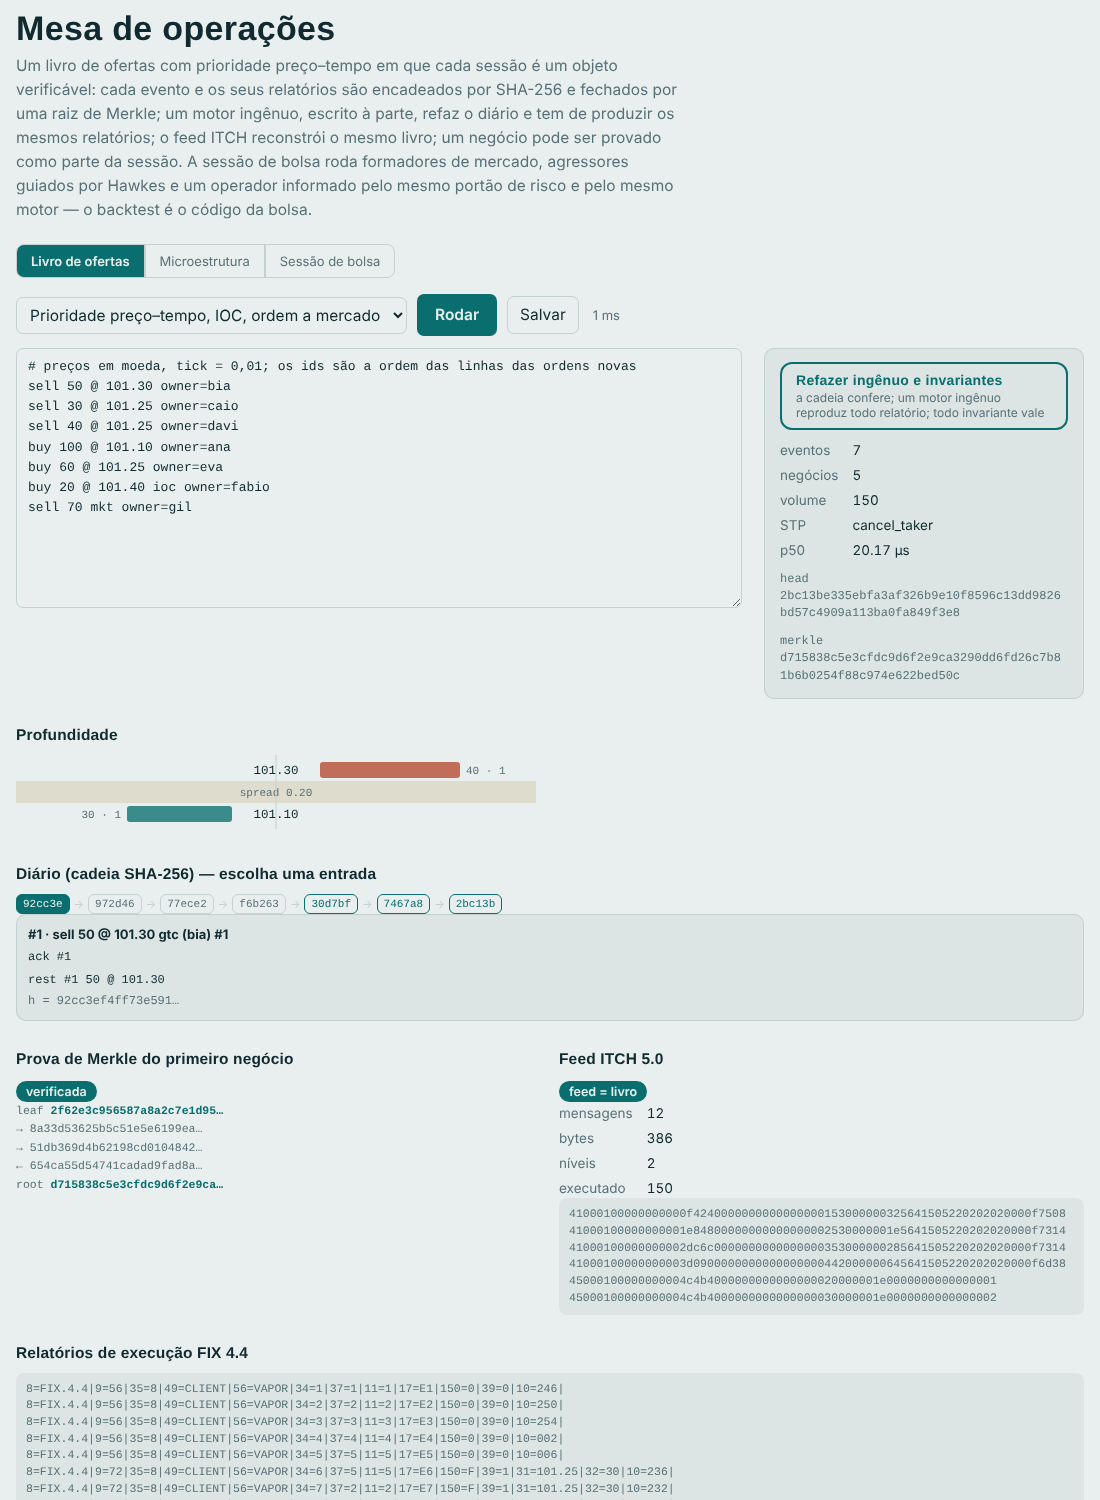
\includegraphics[width=0.82\textwidth]{figuras/console-mesa-livro.png}
\caption{O livro de ofertas no console: profundidade, o diário encadeado (cada entrada selecionável), a prova de Merkle do primeiro negócio, o feed ITCH e os relatórios FIX.}
\label{fig:fin-livro}
\end{figure}

% ----------------------------------------------------------------------------
\section{Protocolos e risco pré-negociação}\label{sec:fin-protocolos}

\paragraph{ITCH 5.0.} Codificador e decodificador das mensagens S, R, A, F, E, C, X, D, U e P da especificação da Nasdaq \cite{itch50}, com os comprimentos exatos (12 a 44 bytes, \textit{big-endian}, preço com 4 casas implícitas, \textit{timestamp} de 6 bytes em nanossegundos). A sessão gera o feed que uma bolsa publicaria, e \code{rebuild/1} reconstrói o livro \emph{só a partir do feed} --- que tem de ser igual ao do motor, nível a nível, e com o mesmo volume executado: um terceiro certificado independente (o feed só vê o que repousa; o motor vê tudo).

\paragraph{FIX 4.4.} Mensagens tag=valor com \textit{BodyLength} (9) e \textit{CheckSum} (10) conferidos na leitura e calculados na escrita --- iguais ao \code{simplefix} byte a byte \cite{fix44}. \textit{NewOrderSingle}, \textit{OrderCancelRequest} e \textit{OrderCancelReplaceRequest} viram eventos do livro; os relatórios viram \textit{ExecutionReports} com numeração própria.

\paragraph{Risco pré-negociação.} O que a Regra 15c3-5 da SEC \cite{sec15c35} e o RTS~6 da MiFID~II \cite{rts6} pedem a quem tem acesso ao mercado --- \emph{e que possa mostrar que tinha}: quantidade máxima (``dedo gordo''), nocional máximo, colar de preço contra a referência, posição máxima no pior caso (executado + ordens abertas daquele lado + esta), taxa de mensagens numa janela e \textit{kill switch}. Uma recusa nunca chega ao livro e \emph{entra no diário} com a causa. O verificador refaz posições, ordens abertas, referências e contagens a partir do diário e confere que nenhuma ordem aceita violou um limite \emph{e que toda recusa teve a causa dita}. O controle atribui a uma recusa por quantidade a causa ``colar de preço'', e é pego.

% ----------------------------------------------------------------------------
\section{Microestrutura, cada modelo com a medida que diz se serve}\label{sec:fin-micro}

\paragraph{Hawkes.} Chegadas que se excitam, com intensidade $\lambda(t) = \mu + \sum_{t_i < t} \alpha e^{-\beta(t - t_i)}$ \cite{hawkes1971,bacry2015}: simulação por \textit{thinning} de \citeonline{ogata1981}, máxima verossimilhança pela recursão $O(n)$, e o \textbf{teste de reescala do tempo}: sob o modelo certo, os incrementos do compensador $\Lambda(t_i) - \Lambda(t_{i-1})$ são Exp(1), julgados por Kolmogorov--Smirnov. Plantado $(\mu, \alpha, \beta) = (1;\, 0{,}6;\, 1{,}5)$, ajustado $(1{,}08;\, 0{,}61;\, 1{,}69)$, razão de ramificação $0{,}36$ (plantada $0{,}40$), KS $p = 0{,}73$. O controle --- um Poisson ajustado às mesmas chegadas --- tem $p = 1{,}7 \cdot 10^{-20}$ (\autoref{fig:fin-hawkes}).

\begin{figure}[htbp]
\centering
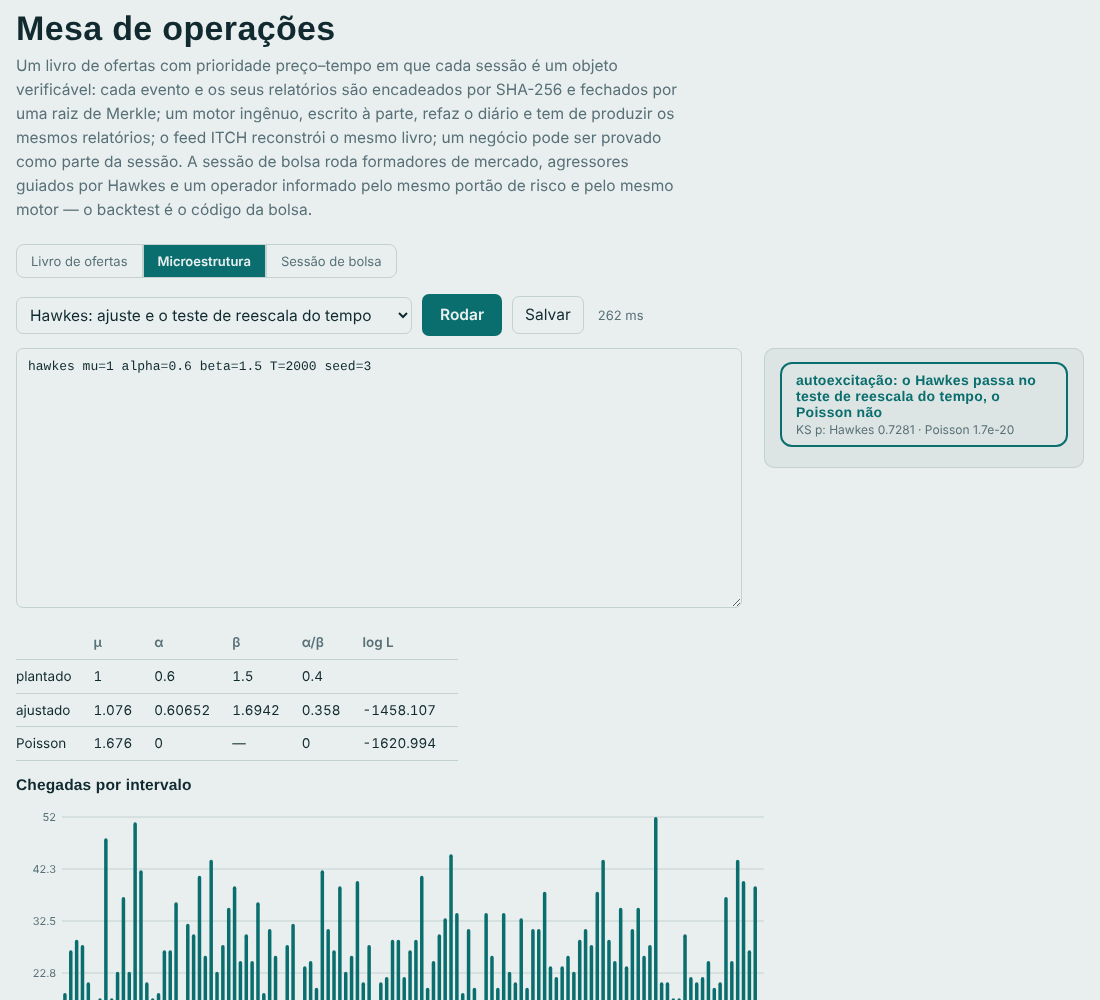
\includegraphics[width=0.78\textwidth]{figuras/console-mesa-hawkes.png}
\caption{Hawkes: os parâmetros plantados e ajustados, o Poisson como controle e o teste de reescala do tempo.}
\label{fig:fin-hawkes}
\end{figure}

\paragraph{Avellaneda--Stoikov.} O formador de mercado de \citeonline{avellaneda2008} cota em torno do preço de reserva $r = s - q\gamma\sigma^2(T - t)$ com \textit{spread} total $\gamma\sigma^2(T-t) + \frac{2}{\gamma}\ln(1 + \frac{\gamma}{k})$. A simulação do §4 do artigo ($s_0 = 100$, $T = 1$, $\sigma = 2$, $dt = 0{,}005$, $k = 1{,}5$, $A = 140$, 1\,000 trajetórias, $\gamma = 0{,}1$) dá, daqui contra o artigo, $\sigma(\text{P\&L})$ de 6,44 / 5,89 para a estratégia de estoque e 13,57 / 13,43 para a simétrica. O \textit{spread} médio daqui (1,49) inclui o termo $\gamma\sigma^2(T-t)$ que a tabela do artigo parece omitir (1,29 é só o segundo termo) --- dito, não escondido.

\paragraph{Almgren--Chriss.} A trajetória ótima de liquidação $x_j = X \sinh(\kappa(T - t_j))/\sinh(\kappa T)$ \cite{almgren2000}, com $\kappa$ da relação discreta $\cosh(\kappa\tau) = 1 + \tilde\kappa^2\tau^2/2$, é \emph{certificada} resolvendo o mesmo problema de média--variância numericamente (um sistema tridiagonal): diferença relativa $10^{-16}$.

% ----------------------------------------------------------------------------
\section{Uma sessão de bolsa que se audita}\label{sec:fin-sessao}

A sessão de bolsa junta tudo: formadores de mercado cotando \textit{post-only} pela regra de Avellaneda--Stoikov em torno do preço público do passo anterior; agressores de ruído cujas chegadas seguem um Hawkes exato em tempo contínuo; um operador informado que conhece o fundamental e agride quando o livro se afasta dele. Toda ordem passa pelo mesmo portão pré-negociação e pelo mesmo motor que uma implantação usaria --- \textbf{o \textit{backtest} é o código da bolsa}, não um modelo dela.

A sessão devolve a própria auditoria (\autoref{fig:fin-sessao}): o diário conferido pelo motor ingênuo, os limites conferidos a partir do diário, o feed ITCH reconstruindo o mesmo livro, e a mesma semente reproduzindo a mesma cabeça de \textit{hash}. E a microestrutura medida na fita recupera o que foi plantado: o ajuste de Hawkes das chegadas acha a autoexcitação (ramificação 0,37 contra 0,40; o Poisson rejeitado), e o \textit{spread} de Roll (5,66) fica próximo do cotado (5,85).

\begin{figure}[htbp]
\centering
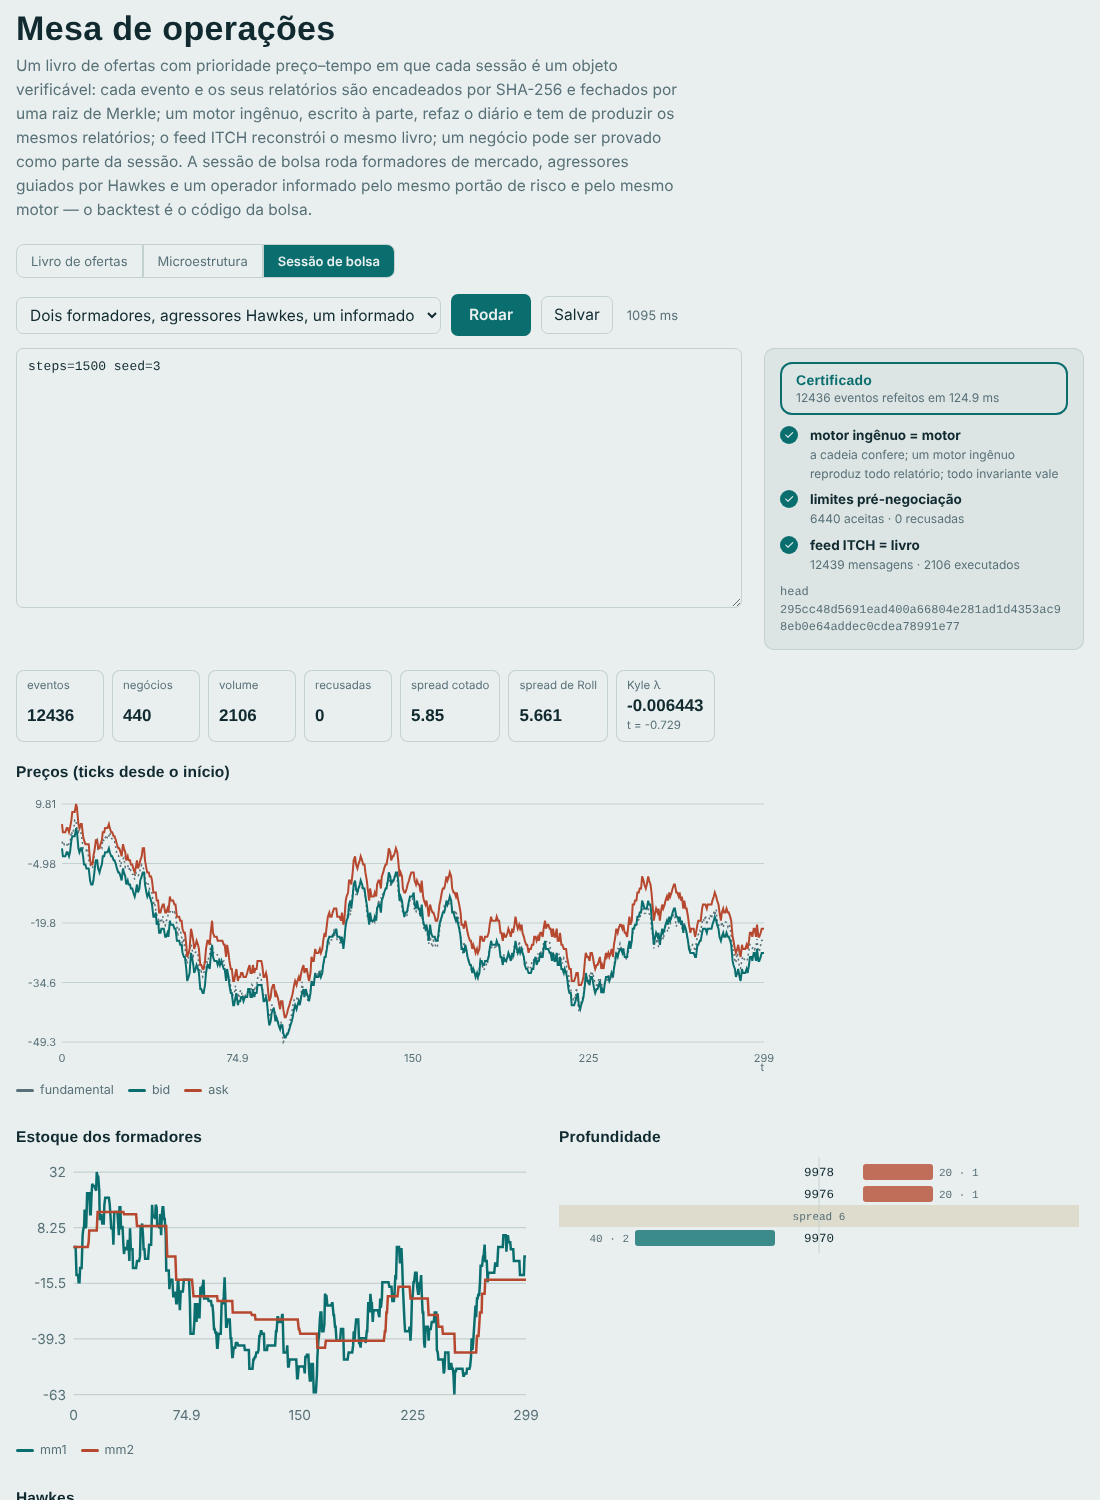
\includegraphics[width=0.82\textwidth]{figuras/console-mesa-sessao.png}
\caption{Uma sessão de 1\,500 passos: 12\,436 eventos refeitos pelo motor ingênuo, limites pré-negociação conferidos, feed ITCH igual ao livro; preços, estoques dos formadores e profundidade.}
\label{fig:fin-sessao}
\end{figure}

\begin{doutorado}
\textbf{Simuladores de mercado verificáveis.} Simuladores baseados em agentes \cite{byrd2020} são usados para treinar e avaliar estratégias, mas o seu motor de casamento raramente é o de uma bolsa real, e os resultados raramente são reproduzíveis entre versões. A sessão do \vapor{} mostra que é possível ter as duas coisas --- o motor de produção e a reprodutibilidade por \textit{hash} ---, mas numa escala de microssegundos. Ficam em aberto: (i) se o motor, compilado como programa canônico ou escrito no worker, pode chegar à escala de nanossegundos mantendo o diário e o juiz fora do caminho crítico; (ii) como calibrar os agentes a dados reais de alta frequência de modo que a microestrutura medida (Hawkes, Roll, Kyle, assinatura da variância) seja um teste de aderência do simulador, e não só uma ilustração.
\end{doutorado}

% ----------------------------------------------------------------------------
\section{O que este capítulo não afirma}\label{sec:fin-limites}

\begin{itemize}
  \item \textbf{Latência de bolsa.} O motor roda na BEAM: microssegundos por evento com \textit{hash}, não nanossegundos. O que se afirma é a verificabilidade e a identidade entre \textit{backtest} e motor.
  \item \textbf{Dados reais.} Nenhum arquivo ITCH da Nasdaq e nenhuma curva da ANBIMA foram usados; os preços dos exemplos são ilustrativos. Os formatos são os das especificações e as convenções as publicadas; os oráculos são o QuantLib, o \code{simplefix}, o SciPy e o ngspice, não os dados.
  \item \textbf{Conselho de investimento.} Os portões dizem quando um \textit{backtest} é indistinguível de ruído; passar neles não torna uma estratégia lucrativa (custos reais, capacidade, mudança de regime).
  \item \textbf{Modelos completos de mercado.} Não há XVA, modelos de taxa de juros de vários fatores (Hull--White, LMM), volatilidade local ou estocástica calibrada a uma superfície inteira, nem crédito.
\end{itemize}
